\section{Real-Clip Planner Visualization}
\label{app:real-clip-planner}

Figures~\ref{fig:planner-trace-real-clip}
and~\ref{fig:planner-examples-gallery} visualize the real-clip budget behind
the Qwen routing frontier in Section~\ref{sec:routing-mechanism}. That result
is a fixed-backend quality--compute claim: the audited policy preserves answer
quality while spending fewer effective fresh frames. These figures show how
local active-region blocks are classified as reusable or fresh before they are
summarized into that effective visual budget. They are not C-PERSIST timing
results and not semantic-saliency maps. Static and shifted blocks are treated
as reusable until the age bound requires refresh; fresh blocks are newly bought
visual evidence. The main text keeps this separate from C-PERSIST and C-VISION
because those regimes have different denominators and validation gates.

\begin{figure}[H]
  \centering
  \IfFileExists{generated/figures/fig1_appendix_broadened/planner_trace_real_clip.pdf}{
    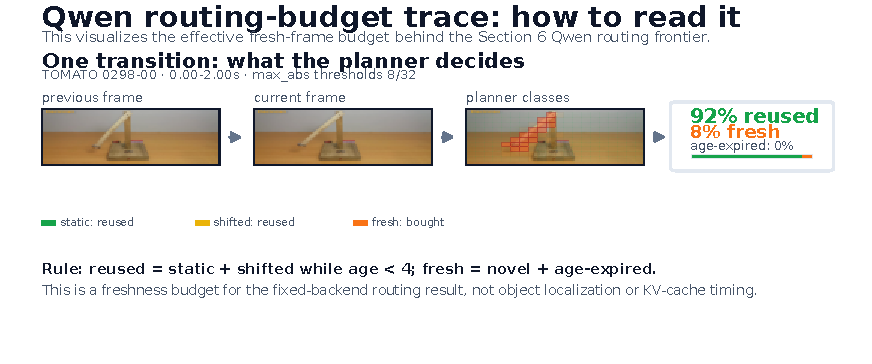
\includegraphics[width=\linewidth]{generated/figures/fig1_appendix_broadened/planner_trace_real_clip.pdf}
  }{
    \fbox{\parbox{0.9\linewidth}{Real-clip planner trace unavailable in this source snapshot.}}
  }
  \caption{Planner trace for one real transition from the Qwen routing budget.
  The figure walks from the previous frame to the current frame, overlays the
  actual static, shifted, and fresh block classes, then summarizes the decision
  as reused versus fresh active-region budget. The rule is shown in the figure:
  static and shifted blocks are reused while their age is below four, while
  novel or age-expired blocks are bought fresh.}
  \label{fig:planner-trace-real-clip}
\end{figure}

\begin{figure}[H]
  \centering
  \IfFileExists{generated/figures/fig1_appendix_broadened/planner_examples_gallery.pdf}{
    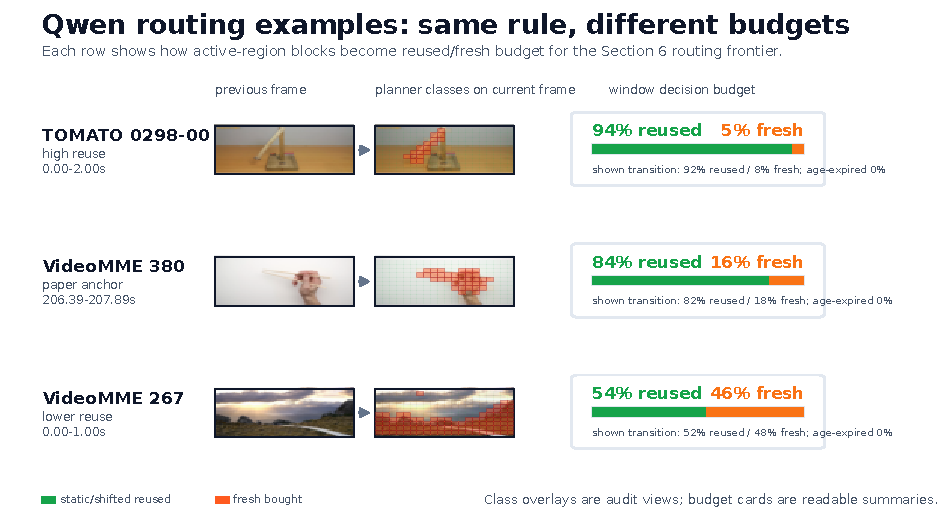
\includegraphics[width=\linewidth]{generated/figures/fig1_appendix_broadened/planner_examples_gallery.pdf}
  }{
    \fbox{\parbox{0.9\linewidth}{Real-clip planner examples unavailable in this source snapshot.}}
  }
  \caption{Same Qwen routing policy over short real windows. Each row selects
  the transition with the strongest fresh signal in that window, shows the
  class overlay on the current frame, and reports the window-average reused
  versus fresh active-region budget. The TOMATO row is a clean high-reuse case,
  the VideoMME 380 row anchors the visualization in the paper protocol, and the
  lower-reuse VideoMME row shows why class overlays are audit views rather than
  headline overview evidence.}
  \label{fig:planner-examples-gallery}
\end{figure}
